\documentclass{article}
\usepackage[utf8]{inputenc}

\title{AREP Lab 1}
\author{Andres Villlamil }
\date{January 2020}

\usepackage{natbib}
\usepackage{graphicx}

\begin{document}

\maketitle

\section{Introduction}
This laboratory intended us to provide the mean and the standard deviation of a given set of doubles. To achieve this, I made my own implementations of linked list and node. This document intends to explain the implementations of this objects.




\subsection{Linked List}
The linked list  is a list that can hold any kind of value, as it is a generic implementation. Each node that make the linked list has a pointer to
the next and the previous nodes to it.
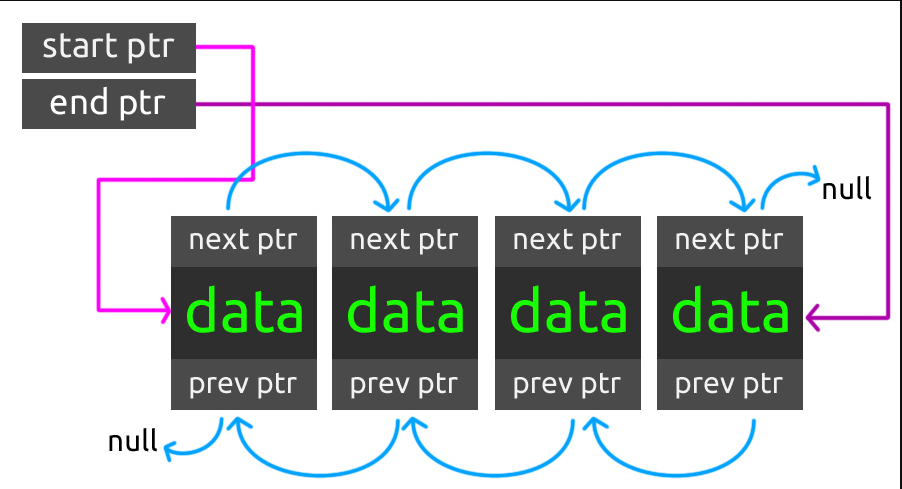
\includegraphics[width=\linewidth]{resources/img/linkedlist.png}

It has 3 attributes
\begin{enumerate}
    \item The size of the linked list.
    \item The head of the linked list.
    \item The tail of the linked list.
\end{enumerate}
\subsubsection{Size}
An int that holds how many items the linkedlist has.
\subsubsection{Head}
A reference indicating which Node is the first of the linked list
Has public getters and setters
\subsubsection{Tail}
A reference indicating which Node is the last of the linked list
Has public getters and setters


\subsection{Node}
The Node is implementation is a generic one
It has 3 attributes:
\begin{enumerate}
    \item The value that the node holds.
    \item The next node.
    \item The previous node.
\end{enumerate}

\subsubsection{Value}
Because of the generic implementation of the node, the value can be any java object.
This attribute has it's public getters and setters

\subsubsection{Next node}
Each node knows which nodes is the next one to them, and stores a reference to that node.
This attribute has it's public getters and setters
\subsubsection{Previous Node}
Each node knows which nodes is the previous one to them, and stores a reference to that node.
This attribute has it's public getters and setters







\bibliographystyle{plain}
\bibliography{references}
\begin{list}
    \url{docs.oracle.com/javase/7/docs/api/java/util/LinkedList.html}
    \url{docs.oracle.com/javase/7/docs/api/java/lang/Iterable.html}
\end{list}


\end{document}
